\section{More realistic bow shock models}
\label{sec:more-realistic-bow}

\begin{figure}
  (a)\\
  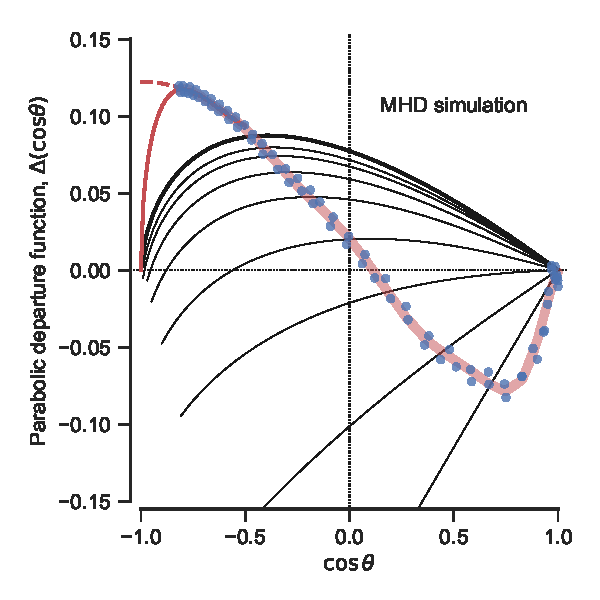
\includegraphics[width=\linewidth]
  {figs/depart-cheby-M17-MHD2040-AllB7}\\[-\baselineskip]
  (b)\\
  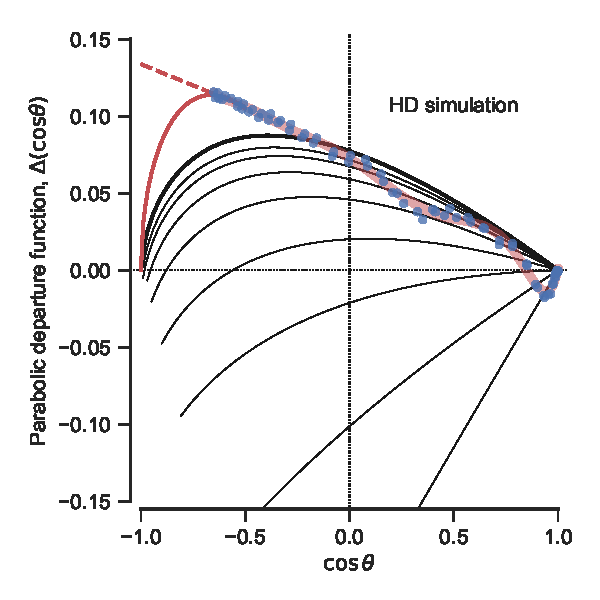
\includegraphics[width=\linewidth]
  {figs/depart-cheby-M17-HD2040}\\[-\baselineskip]
  \caption[]{Departure function for the shape of the contact
    discontinuity, measured from two numerical simulations of a
    \SI{20}{M_\odot} main-sequence star, moving at \SI{40}{km.s^{-1}}
    through a uniform medium of density \SI{0.57}{cm^{-3}}
    \citep{Meyer:2017a}. (a)~Magnetohydrodynamic simulation with
    ambient magnetic field of strength \SI{7}{\micro G}, oriented
    parallel to the stellar velocity. (b)~Hydrodynamic simulation with
    zero magnetic field.  Blue dots show the measured shape, while the
    thick, pale-red line shows a 12th-order Chebyshev polynomial fit.
    The published shapes only extend to
    \(\theta \approx 130\)--\ang{150}, so we extrapolate the shapes out to
    \(\theta = \ang{180}\). Two different extrapolations are shown,
    corresponding to bows that are asymptotically closed (dashed red
    line) or open (solid red line).  For comparison, black lines show
    the departure function for wilkinoid (thick line) and cantoids
    (thin lines).}
  \label{fig:sim-depart}
\end{figure}

The assumptions underlying the models of the previous section may
break down in various ways.  To test whether the planitude--alatude
analysis is still useful in less ``ideal'' situations, we here apply
it to more realistic simulations of stellar bow shocks.  We choose a
pair of hydromagnetic (HD) and magnetohydrodynamic (MHD) moving-star
simulations from \citet{Meyer:2017a}, in which the only difference is
the presence (MHD case) or absence (HD case) of an ambient magnetic
field with strength \(B = \SI{7}{\micro G}\), oriented parallel to the
stellar velocity.  In each case, the inner wind comes from a
\(20\,M_\odot\) main-sequence star, with mass loss rate and terminal
velocity that are roughly constant with time at
\(\dot{M}_{\w} \approx \SI{4e-7}{M_\odot.y^{-1}}\) and
\(V_{\w} \approx \SI{1200}{km.s^{-1}}\), while the outer wind is a
parallel stream due to the star's own motion at \SI{40}{km.s^{-1}}
through a uniform medium of density \SI{0.57}{cm^{-3}}.

For these parameters, the radiative cooling distance for shocked
ambient gas in the bow is a significant fraction (\(\approx 10\%\)) of the
bow shock size, \(R_0\), tending to increase towards the wings, and
the radiative cooling in the shocked stellar wind is even less
efficient.  This represents a gross violation of the assumptions
behind the thin-shell models, since the total shocked shell thickness
is of the same order as \(R_0\).  The parabolic departure function
(see \S~\ref{sec:parab-depart-funct}) for the shape of the contact
discontinuity\footnote{%
  Note that, in the non-magnetic HD models, efficient thermal
  conduction leads to a thick layer of hot, thermally evaporated
  ambient material that separates the shocked stellar wind from the
  cool, dense shell of shocked ambient gas \citep[see \S~3.3
  of][]{Meyer:2014b}.  In this case, the contact discontinuity is
  taken to be the boundary between hot and cold ambient gas, as
  opposed to the \textit{material discontinuity} between shocked
  ambient gas and shocked wind gas.  In the MHD models, the thermal
  conduction is almost completely suppressed, so that the material and
  contact discontinuities coincide. } %
in the two models is shown in Figure~\ref{fig:sim-depart} as blue
symbols.\footnote{%
  Measured from Figure~3 of \citet{Meyer:2017a} by tracing the
  \SI{0.4}{cm^{-3}} density contour.} %
The MHD simulation shows a strongly negative dip in the departure
function close to the apex (\(\cos \theta = 1\)), indicating a very flat
shape.\footnote{%
  \citet{Meyer:2017a} speculate that this flatness may be the
  signature of the formation of a complex multiple-shock topology at
  the apex \citep{de-Sterck:1999a}.  For our purposes, the reason does
  not matter, merely that the magnetic and non-magnetic models predict
  markedly different shapes. } %
The HD simulation shows only a small negative dip in the departure
function at the apex, but otherwise approximately follows the
wilkinoid curve in the forward hemisphere.  In both cases the
departure function is more positive than the wilkinoid in the far
wings (\(\cos \theta < -0.5\)), but we do not have data for the full range
of \(\theta\), and so two different extrapolations for
\(\theta \to \ang{180}\) are shown.  In the first (dashed red line in
figure), we fit a low-order polynomial of \(\cos \theta\) to the points
with \(\cos \theta < -0.5\) and extend it to \(\cos \theta = -1\), which gives
an asymptotically closed shape.  In the second extrapolation (solid
red line in figure), we fit a polynomial that is multiplied by
\((1 + \cos\theta)^{1/2}\), which forces the departure function to zero at
\(\cos \theta = -1\), giving an asymptotically open shape, as with the
wilkinoid.  In a true steady state, the far wings should be
asymptotically open, but as \(\theta \to \ang{180}\) the flow times become
longer and longer, so that a bow shock with a finite age will be
closed.

\begin{figure}
  \centering
  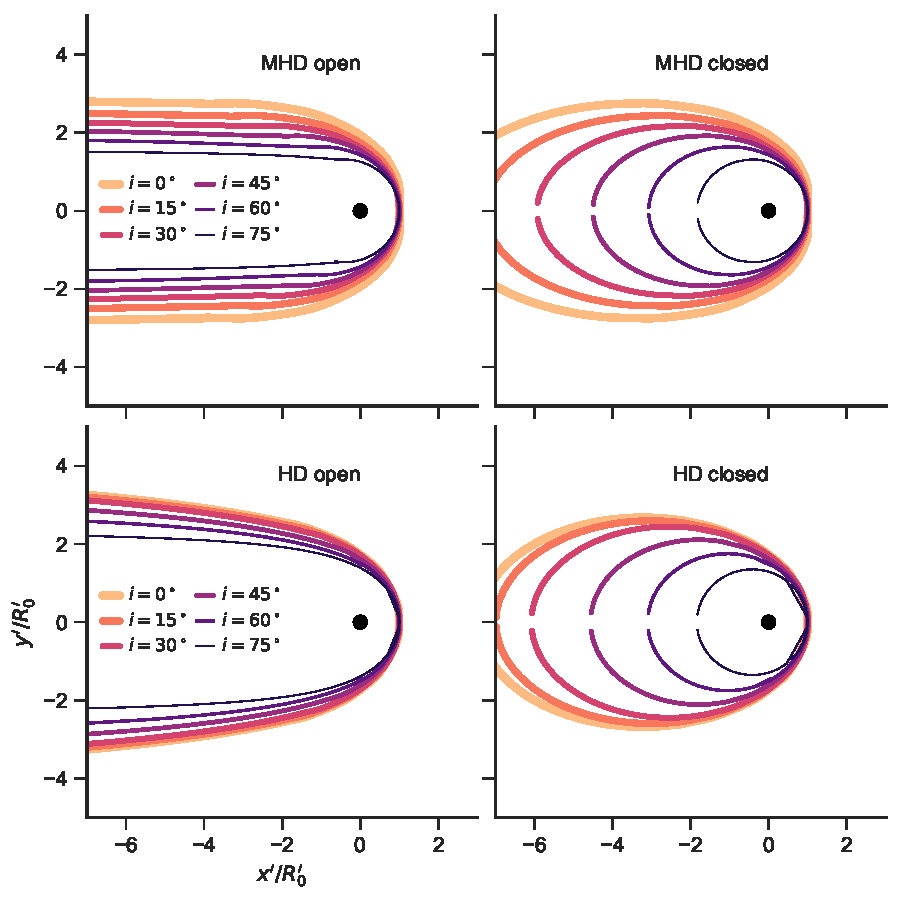
\includegraphics[width=\linewidth]{figs/test_xyprime_simulation}
  \caption[]{Projected shapes of contact discontinuity from
    simulations at different inclinations \(\abs{i}\) (varying line
    color and thickness, see key).  Top row shows magnetized
    simulation of Fig.~\ref{fig:sim-depart}a, bottom row shows
    non-magnetized simulation of Fig.~\ref{fig:sim-depart}b.  Left
    column shows asymptotically open extrapolation, right column shows
    asymptotically closed extrapolation.  All shapes are normalized to
    the projected apex distance, \(R_0'\) }
  \label{fig:sim-xyp}
\end{figure}

Using a 12th-order Chebyshev fit to the traced shapes, we show the
apparent shape of the contact discontinuity at a series of inclination
angles, \(\abs{i}\), in Figure~\ref{fig:sim-xyp}.  The four panels
show the two simulations for each of the two far-wing extrapolations.
Comparison with Figures~\ref{fig:xyprime}
and~\ref{fig:xyprime-ancantoid} shows the general tendency is the same
as with the wilkinoid: that the apex becomes less flat and the wings
less open as the inclination angle is increased.  There is no sign of
the sudden increase in openness at high inclination, as seen in the
cantoids and ancantoids that are asymptotically hyperbolic.  On the
other hand, the projected shapes of both simulations vary much more
strongly with \(\abs{i}\) than the wilkinoid does.  For the HD
simulation, this is mainly apparent for \(\abs{i} > \ang{30}\), but
for the MHD simulation it occurs at all inclinations.


\begin{figure}
  \centering
  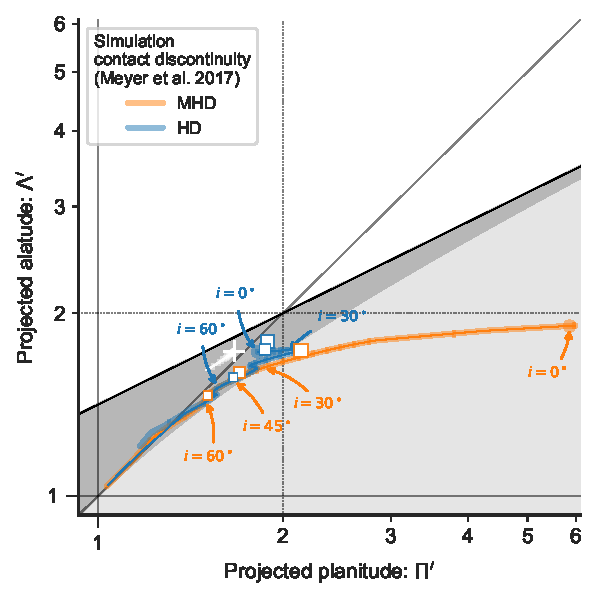
\includegraphics[width=\linewidth]{figs/m17-planitude-alatude}
  \caption[]{Apparent projected shapes of simulations in the
    \(\Pi'\)--\(\Lambda'\) plane.  Thick solid lines show the predicted
    inclination-dependent tracks of the traced contact discontinuity
    shape for the asymptotically open extrapolation, with tick marks
    indicating 20 equal intervals in \(\abs{\sin i}\). Thin solid
    lines show the same for the asymptotically closed extrapolation,
    which only deviates from the open case at the high-\(\abs{i}\) end
    of the HD tracks.  The true planitude and alatude are marked by
    filled circle symbols.  Open square symbols show the shapes traced
    from the dust emission maps at \SI{60}{\um} for inclinations of
    (largest to smallest) \ang{30}, \ang{45}, and \ang{60}. For
    comparison, the wilkinoid track is shown in white. Note that the
    scales of both axes are logarithmic in this case.}
  \label{fig:sim-Pi-Lambda}
\end{figure}

The resultant inclination-dependent tracks in the planitude--alatude
plane are shown in Figure~\ref{fig:sim-Pi-Lambda}.  These are compared
with measurements\footnote{%
  The shape measurements were performed by converting to contours the
  \SI{60}{\um} images in \citet{Meyer:2017a}'s Fig.~10 and then
  tracing the ridge of minimum radius of curvature of the contours.
  Identical results are found from using the \SI{100}{\um} maps
  instead.  For the \SI{25}{\um} maps, although the same results are
  found for low inclinations, in the maps with
  \(\abs{i} \ge \ang{45}\) in the HD case it becomes impossible to trace
  the limb-brightened rim because it becomes fainter than the emission
  from the true apex of the bow.} %
from post-processed infrared dust continuum maps at \SI{60}{\um}
\citep[\S~4.3 of][]{Meyer:2017a}, shown by open square symbols for
\(i = \ang{30}\), \ang{45}, and \ang{60}.  The agreement between the
two is good.  In particular, the \SI{60}{\um}-derived shapes are
always very close to the tracks derived from the contact discontinuity
shape. Also, the ordering of the three inclinations along the tracks
corresponds to what is predicted, although quantitatively there are
some slight deviations.  This close agreement stems for the fact that
the long-wavelength dust emission from hot-star bow shocks tends to be
dominated by material just outside the contact discontinuity, as
emphasized by \citet{Meyer:2014b}.

\begin{figure}
  \centering
  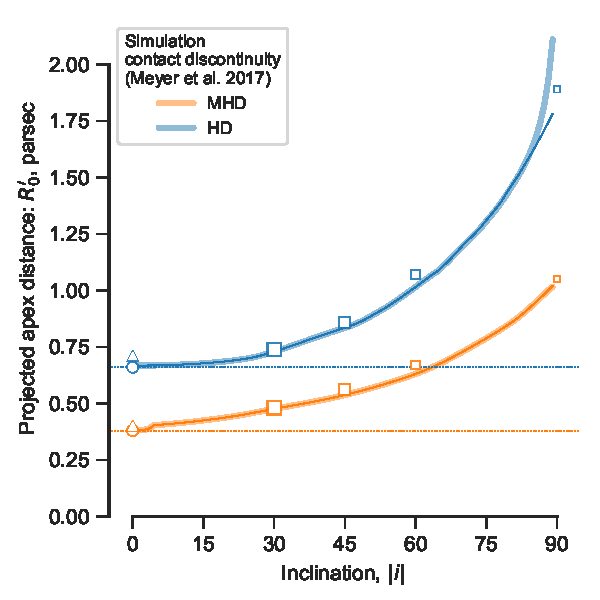
\includegraphics[width=\linewidth]{figs/m17-r0-prime}
  \caption[]{Apparent projected apex distance of simulations.}
  \label{fig:sim-R0-prime}
\end{figure}


\section{Summary and discussion}
\label{sec:conc}

We have shown that the shapes of stellar bow shocks can be usefully
characterized by two dimensionless numbers: the \textit{planitude},
\(\Pi\), or flatness of the bow's apex, and the \textit{alatude},
\(\Lambda\), or openness of the bow's wings.  The planitude and alatude can
be estimated from ratios of lengths that can be straightforwardly
measured from observations or theoretical models.  We develop a
general method for finding the projected shape,
\((\Pi', \Lambda')\), of a bow shock's limb-brightened edge, or
\textit{tangent line}, as a function of inclination angle, \(i\),
where the emission shell is idealized as a cylindrically symmetric
surface.

We first apply this method to find inclination-dependent tracks on the
projected planitude--alatude plane for the special case of
\textit{quadric} surfaces, such as hyperboloids, paraboloids, and
spheroids, where the tangent line is a conic section.  The spheroids
and hyperboloids occupy distinct regions of the plane, with the
paraboloids defining the boundary between the two.  As the inclination
is increased from \(\abs{i} = 0\) (side-on) to \(\abs{i} = \ang{90}\)
(end-on), the tracks first tend to approach the diagonal
\(\Lambda' = \Pi'\), corresponding to confocal conics, always remaining within
their own region.  At the highest inclinations, the spheroids all
converge at \(\abs{i} = \ang{90}\) on the point
\((\Pi', \Lambda') = (1, 1)\) and the paraboloids on the point
\((\Pi', \Lambda') = (2, 2)\).  The hyperboloids, on the other hand diverge as
\((\Pi', \Lambda') \to (\infty, \infty)\) for a finite
\(i_{\mathrm{crit}}\), which depends on the asymptotic opening angle
of the tail.  For \(\abs{i} > i_{\mathrm{crit}}\), the tangent line no
longer exists for the hyperbola, and it no would longer appear to be a
bow shock.

We then apply the projection method to a set of thin-shell
hydrodynamic models of bow shocks: the \textit{wilkinoid} from a
wind-parallel stream interaction and the \textit{cantoids} from
wind-wind interactions.  We generalize the latter to the
\textit{ancantoids}, where one of the winds is anisotropic.  We find
that the wilkinoid is confined to a small region of the
\(\Pi'\)--\(\Lambda'\) plane, with projected planitude and alatude varying with
inclination by \(< 15\%\).  The cantoids and ancantoids with
sufficiently small values of \(\beta\), the wind momentum ratio, have more
interesting behavior, with tracks that pass from the spheroid region
at low inclinations to the hyperboloid region at high inclinations.  

This paper is the first of a series that will apply our shape analysis
to a wide variety of models and observations of stellar bow shocks.
In a second paper \citep{Henney:2018a}, we consider the alternative
model of dusty radiation-driven bow wave, instead of a hydrodynamic
bow shock, and also calculate the signature in the planitude--alatude
plane of oscillations in the bow shape, which may be due to
instabilities or a time-varying source.  In a third paper
\citep{Henney:2018b}, we apply our techniques to observational
datasets for three different classes of stellar bow shocks: OB stars,
cool giants/supergiants, and young stars in the extended Orion Nebula.
In a fourth paper \citep{Tarango-Yong:2018b}, we analyze the proplyd
bow shocks in the core of the Orion Nebula.


%and was applied to the proplyds in the core of the ONC.
%We started measuring the projected characteristic radii $(R'_0,R'_c)$ for each proplyd in our
%sample and compare them with the ``conic equivalent'' of a two winds interaction model based 
%on \CRW{} work to estimate the intrinsic bow shock shape and get the ionizing flux for ionization balance 
%and the stagnation pressure for our sample of proplyds.
%Most results are consistent with a proplyd's photoevaporated flow with an anisotropic density
%distribution, with different anisotropy degrees. We ound that LV4 has the least anisotropic flow,
%while LV2 has the most anisotropic flow. And for the 177-341, 169-348 and 180-331 we found out that 
%the stellar wind is not enough to keep their bow socks stationary.

%%% Local Variables:
%%% mode: latex
%%% TeX-master: "quadrics-bowshock"
%%% End:
